% Scalar instruction entry source: tools/generate_scalar_instruction_catalog.py.
\subsection{\texttt{SD.U}}
\label{sec:scalar-sd_u}
\index{SD.U@\texttt{SD.U}}
\begin{sloppypar}\noindent\textbf{Purpose.} Stores a 64-bit value to memory using unscaled register-offset addressing.\end{sloppypar}\smallskip
\noindent\textbf{Syntax.}\par
\begin{lstlisting}[style=ptoscalarcode]
sd.u SrcD, [SrcL, SrcR<{.sw,.uw,.neg}>]
\end{lstlisting}
\noindent\textbf{Encoding.}\par
\noindent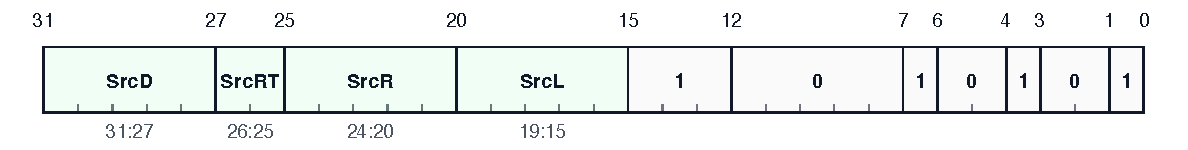
\includegraphics[width=\textwidth]{figs/encoding/scalar_instruction_entries/enc_sd_u.pdf}\par\smallskip
\begin{description}[leftmargin=0.18\linewidth,style=nextline]
\item[Format] \texttt{L32} \texttt{32-bit} scalar word.
\item[Pattern] \texttt{.................111000001001001}.
\end{description}
\noindent\textbf{Classification.}\par
\begin{description}[leftmargin=0.18\linewidth,style=nextline]
\item[Category] Load, Store, and Address Generation.
\item[Family] Store Register Offset.
\item[Execution class] \texttt{STA/BASE\_REG}; uop\_kind=AGU, agu\_kind=STA, addr\_mode=BASE\_REG, split=AGU+STD.
\end{description}
\noindent\textbf{Operand fields.}\par
\begin{description}[leftmargin=0.18\linewidth,style=nextline]
\item[\texttt{SrcD}] Bits \texttt{31:27 (5b)}. 5-bit scalar source register containing the data value written to memory; the instruction size selects the stored byte, halfword, word, or doubleword portion.
\item[\texttt{SrcL}] Bits \texttt{19:15 (5b)}. 5-bit scalar source register used as the base address for the memory access.
\item[\texttt{SrcR}] Bits \texttt{24:20 (5b)}. 5-bit scalar source register used as the register offset component of the effective address.
\item[\texttt{SrcRType}] Bits \texttt{26:25 (2b)}. 2-bit modifier for SrcR. It selects the encoded source form shown in the syntax, such as signed-word, unsigned-word, negated, or unmodified register input.
\end{description}
\noindent\textbf{Operation.}\par
\begin{lstlisting}[style=ptoscalarcode]
addr = ComputeAddress(/* per syntax */)
Store64(addr, Read(SrcD))
\end{lstlisting}
\Needspace{0.08\textheight}
